\documentclass[aspectratio=169,
				xcolor=table]{beamer}

% Load general definitions
\usepackage[utf8]{inputenc}
%\usepackage[T1]{fontenc}
\usepackage[brazil]{babel}
\usepackage{amsmath}
\usepackage{amsfonts}
\usepackage{amssymb}
\usepackage{graphicx}
\usepackage{verbatim}
\usepackage{cancel}
\usepackage{askmaps}
\usepackage{tabularx}
\usepackage[table]{xcolor}
%\usepackage{tikz}
\usepackage{multirow}
\usepackage{mathtools}
\usepackage{color, colortbl}
\usepackage{etoolbox}
\usepackage{pbox}
\usepackage{changepage}
\usepackage{xpatch}
\usepackage{array}
\usepackage{marvosym}
\usepackage{tabu}
\usepackage{multicol}
\usepackage{listings}
\usepackage{underscore}
\usepackage{filecontents}
\usepackage[]{algorithm2e}
\usepackage{ragged2e}

\newcolumntype{P}[1]{>{\centering\arraybackslash}m{#1}}
\definecolor{Gray}{gray}{0.75}
\definecolor{Gray2}{gray}{0.85}

\definecolor{lightBlue}{HTML}{DAE8FC}
\definecolor{Blue}{RGB}{51, 51, 204}

%\useinnertheme[lily]{rounded}
\usetheme{UniEvangelica}
%\usetheme{Copenhagen}
%\usetheme{Berlin}
%\usecolortheme{dolphin}
\tolerance=1
\emergencystretch=\maxdimen
\hyphenpenalty=10000
\hbadness=10000

\setbeamertemplate{navigation symbols}{}%remove navigation symbols


\let\olditem=\item% 
\renewcommand{\item}{\olditem \justifying}%
\def\center{\trivlist \centering\item\relax}
\def\endcenter{\endtrivlist}

\setbeamertemplate{itemize/enumerate body begin}{\large}
\setbeamertemplate{itemize/enumerate subbody begin}{\large}

\setbeamertemplate{itemize item}{\raisebox{0.1ex}{$\blacktriangleright$}\hskip0.1em}
\setbeamertemplate{itemize subitem}{\raisebox{0.1ex}{$\blacktriangleright$}\hskip0.1em}

\newcommand{\greenarrow}{\textcolor{green}{\rotatebox[origin=c]{180}{\MVArrowDown}}}

\newcommand{\redarrow}{\textcolor{red}{\MVArrowDown}}

%\newcommand{\ftable}{
%	\begin{table}
%		\large
%		\centering
%		\rowcolors{1}{\ifnumless{\rownum}{2}{Blue}{lightBlue}}{}
%}

\newenvironment{eftable}{
	\begin{table}
		\large
		\centering
		\rowcolors{1}{}{Blue}
		\rowcolors{1}{\ifnumless{\rownum}{2}{Blue}{lightBlue}}{}
	}
	{
	\end{table}
}


%\setbeamertemplate{frametitle}
%{
%	%\vspace*{-2em}	
%	\insertframetitle
%
%	 %\textcolor{white}{\LARGE \insertframetitle}
%
%}

% Specific definitions
\institute[]{\uppercase{Engenharia de Software}}
\title[]{Sistemas Operacionais}
\subtitle[]{Deadlocks}
\author[]{Prof. M.e Alexandre Tannus}
\date{Anápolis - 2021.1}

\AtBeginSection{\frame{\tableofcontents[currentsection]}}
\begin{document}
	
	\begin{frame}
		\titlepage
	\end{frame}

	\begin{frame}
		\tableofcontents
	\end{frame}		
	
	\begin{frame}{Questionamentos}
		\begin{itemize}
			
			\item O que fazer se vários processos quiserem o mesmo recurso?
			\vspace{1em}
			\item E se não houver como liberar o recurso?
			\vspace{1em}
			\item Quais estratégias são interessantes para destravar um recurso e evitar a inanição de um processo?
		\end{itemize}
	\end{frame}
	
	\section{Introdução}
	\begin{frame}{Relembrando...}
		\alert{Condições de corrida}
		\begin{itemize}			
			\item Situações onde dois os mais processos estão lendo ou escrevendo algum dado compartilhado e o resultado depende de quem processa no momento propício.
		\end{itemize}
			\vspace{1em}
			\begin{figure}
				\centering
				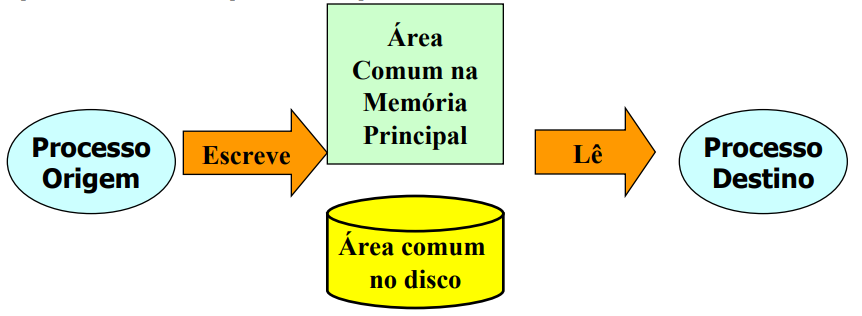
\includegraphics[keepaspectratio, height=0.5\paperheight]{../figs/cap05/race1.png}			
			\end{figure}

	\end{frame}

	\begin{frame}{Relembrando...}
		\alert{Formas de Escalonamento}
		\begin{itemize}
			\item Não Preemptivo
			\begin{itemize}
				\item Execução de um processo selecionado até
				\begin{itemize}
					\item Finalização do processo
					\item Bloqueio do processo por E/S
					\item Liberação voluntária da CPU pelo processo
				\end{itemize}
			\end{itemize}
			\vspace{1em}			
			\item Preemptivo
			\begin{itemize}
				\item Execução de um processo selecionado por um tempo fixo
				\item Suspensão do processo ao final do tempo e seleção de outro processo para execução
			\end{itemize}
		\end{itemize}	
	\end{frame}
	
	\begin{frame}{Situação Problema}
		\begin{itemize}
			\item Ivan reserva uma sala para ensinar os colegas, mas não possui marcadores de quadro e cabos para ligar os equipamentos.
			\vspace{1em}
			\item Marta possui marcadores de quadro e cabos para ligar os equipamentos, mas não tem acesso à sala.
		\end{itemize}
		\vspace{2em}
		\Huge \centering \alert{Como resolver o problema?}
	\end{frame}

	\begin{frame}{Recursos}
		\begin{itemize}
			\item Dispositivos de \textit{hardware} ou \textit{software} disponibilizados pelo sistema operacional.
			\vspace{1em}
			\item Conjunto finito.
			\vspace{1em}
			\item Apenas um processo pode utilizar o recurso em um dado instante.
		\end{itemize}
	\end{frame}	

	\begin{frame}{Situação Problema - Recursos e Processos}
		\begin{itemize}
			\item Recursos
			\begin{itemize}
				\item Marcadores de quadro e cabos
				\item Sala de aula
			\end{itemize}
			\vspace{1em}
			\item Processos
			\begin{itemize}
				\item Ivan
				\item Marta
			\end{itemize}
		\end{itemize}			
	\end{frame}	
	
	\begin{frame}{Tipos de recursos}
		\begin{itemize}
			\item Preemptivo
			\begin{itemize}
				\item Pode ser retirado do processo sem efeito prejudicial
				\begin{itemize}
					\item Memória
				\end{itemize}
			\end{itemize}
			\vspace{1em}
			\item Não preemptivo
			\begin{itemize}
				\item Não pode ser retirado do proprietário sem causar falhas
				\begin{itemize}
					\item Impressora
					\item Gravador de DVD/CD
				\end{itemize}
			\end{itemize}
		\end{itemize}
	\end{frame}
	
	\begin{frame}{Sequência de eventos}
		\begin{itemize}
			\item Solicitação do recurso
			\vspace{1em}
			\item Utilização do recurso
			\vspace{1em}
			\item Liberação do recurso
		\end{itemize}
	\end{frame}
	
	\begin{frame}{Definição de impasse}
		\begin{block}{Deadlock}
			Um conjunto de processos está em um impasse (\textit{deadlock}) se cada processo do conjunto está esperando por um evento que apenas outro processo do conjunto pode causar.
		\end{block}
	\end{frame}
	
	\section{Condições de existência}
	\begin{frame}{Condições de existência}
		\begin{itemize}
			\item Exclusão mútua
			\begin{itemize}
				\item Um recurso está atribuído a apenas um processo ou disponível para uso
			\end{itemize}
			\vspace{0.5em}
			\item Posse e espera
			\begin{itemize}
				\item Processos com recursos alocados podem solicitar novos recursos
			\end{itemize}
			\vspace{0.5em}
			\item Ausência de preempção
			\begin{itemize}
				\item Recursos garantidos devem ser liberados voluntariamente pelo processo, sem retirada forçada.
			\end{itemize}
			\vspace{0.5em}
			\item Espera circular
			\begin{itemize}
				\item Encadeamento circular entre dois ou mais processos e seus respectivos recursos alocados
			\end{itemize}
		\end{itemize}
	\end{frame}
	
	\begin{frame}{Impasse em potencial}
		
		\begin{figure}
			\centering
			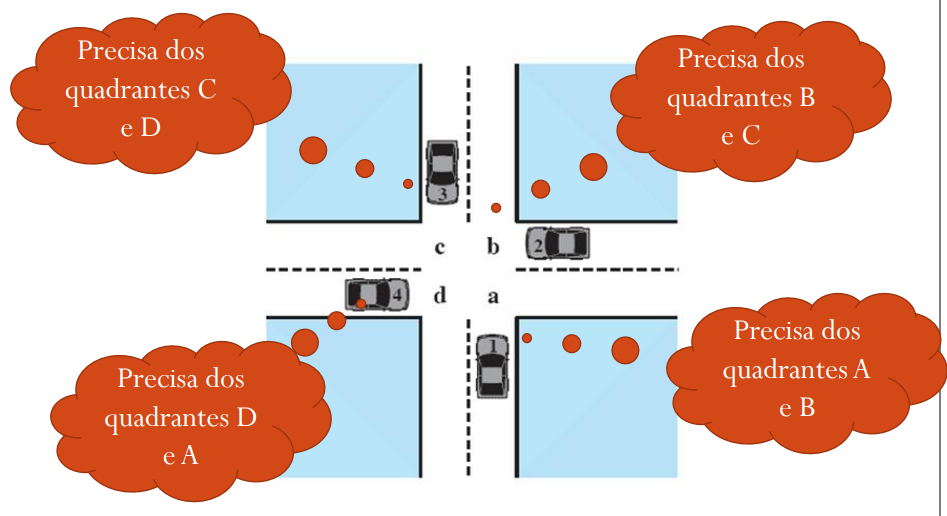
\includegraphics[keepaspectratio, height=0.75\paperheight]{../figs/cap07/potencial.png}			
		\end{figure}
	\end{frame}
	
	\begin{frame}{Impasse real}
		\begin{figure}
			\centering
			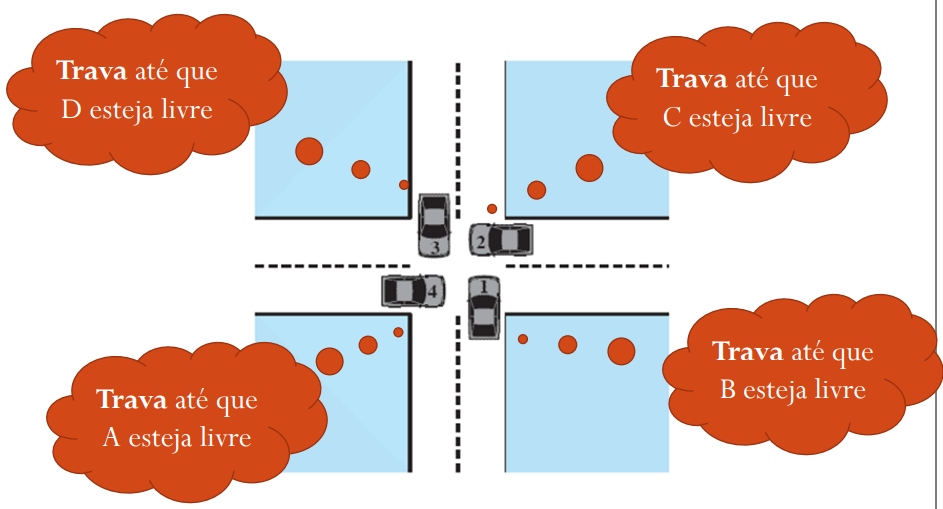
\includegraphics[keepaspectratio, height=0.75\paperheight]{../figs/cap07/real.png}			
		\end{figure}
		
	\end{frame}
		
	\begin{frame}{Modelagem do impasse}
		\begin{itemize}
			\item Grafo de alocação de recursos
		\end{itemize}
		\vspace{2.5em}
		\begin{figure}
			\centering
			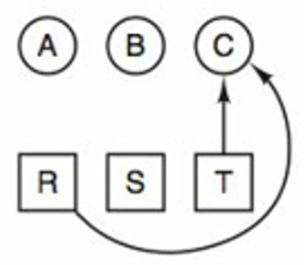
\includegraphics[keepaspectratio, height=0.5\paperheight]{../figs/cap07/grafo01.png}			
		\end{figure}
	\end{frame}
	
	\begin{frame}{Modelagem - Solicitação de recurso}
		
		\begin{figure}
			\centering
			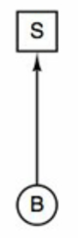
\includegraphics[keepaspectratio, height=0.5\paperheight]{../figs/cap07/solicitacao.png}			
		\end{figure}
	\end{frame}
	
	\begin{frame}{Modelagem - Manutenção de recurso}
		
		\begin{figure}
			\centering
			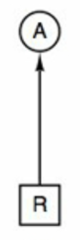
\includegraphics[keepaspectratio, height=0.5\paperheight]{../figs/cap07/manutencao.png}			
		\end{figure}
	\end{frame}
	
	\begin{frame}{Impasse}
		
		\begin{figure}
			\centering
			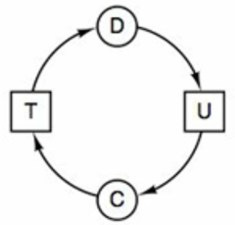
\includegraphics[keepaspectratio, height=0.75\paperheight]{../figs/cap07/impasse.png}			
		\end{figure}
	\end{frame}

	\begin{frame}{Questão}
	
		\begin{block}{}
		Em um sistema computacional multiprocessado, onde o sistema operacional realiza escalonamento de tarefas do tipo preemptivo, três processos (P1, P2 e P3) compartilham recursos (R1, R2 e R3). Os processos P1 e P2 concorrem entre si ao acesso do recurso R1, enquanto P2 e P3 concorrem entre si ao acesso dos recursos R2 e R3. Os recursos R1 e R3 são não preemptíveis e R2 é um recurso preemptível. Todos os três processos usam o mesmo mecanismo de exclusão mútua para garantir acesso exclusivo em suas seções críticas.
		\end{block}
		\vspace{1em}
		\Huge \centering \alert{Existe deadlock?}
	\end{frame}
	
	\begin{frame}
		\begin{figure}
			\centering
			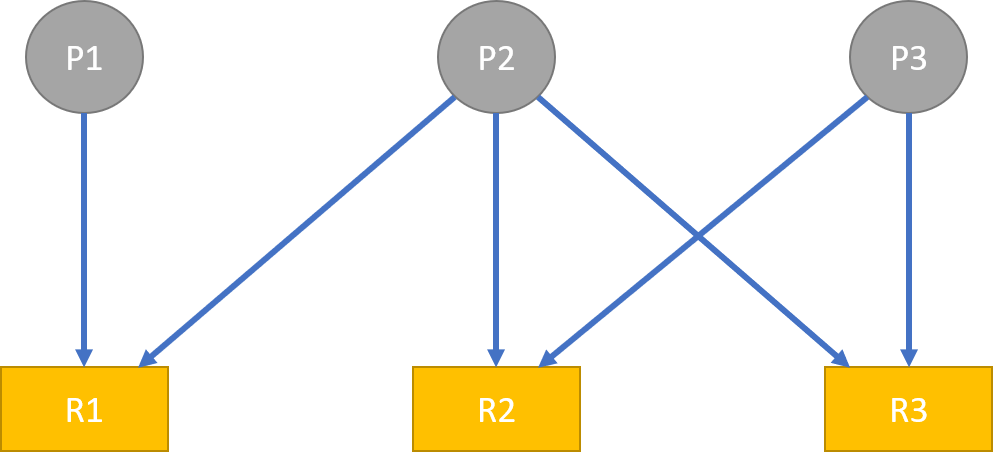
\includegraphics[keepaspectratio, width=0.9\paperwidth]{../figs/cap07/exercicio01.png}			
		\end{figure}		
	\end{frame}
		
	\begin{frame}{Questão - Situação 1}
		\begin{itemize}
			\item Recurso R1 é detido pelo processo P1. Processo P1 deseja recurso R1
		\end{itemize}
		\begin{figure}
			\centering
			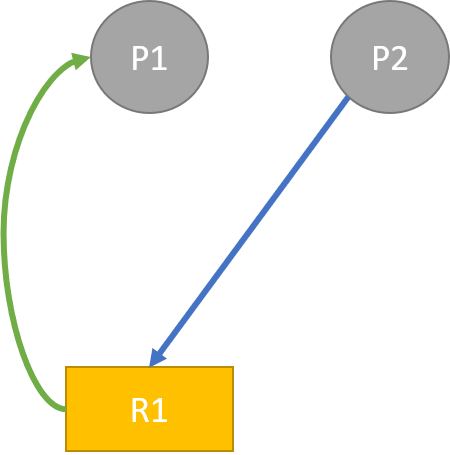
\includegraphics[keepaspectratio, height=0.7\paperheight]{../figs/cap07/exercicio02.png}			
		\end{figure}		
	\end{frame}

		
	\begin{frame}{Questão - Situação 2}
		\begin{itemize}
			\item Recurso R1 é detido pelo processo P2. Processo P1 deseja recurso R1
		\end{itemize}
		\begin{figure}
			\centering
			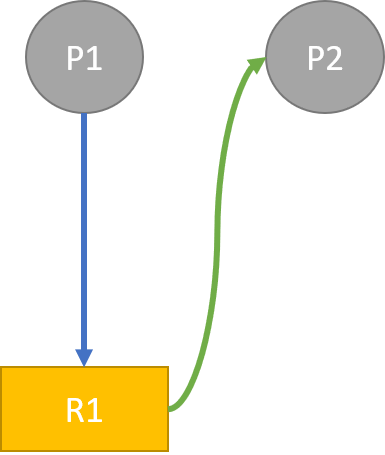
\includegraphics[keepaspectratio, height=0.7\paperheight]{../figs/cap07/exercicio03.png}			
		\end{figure}		
	\end{frame}	
			
	\begin{frame}{Questão - Situação 3}
		\begin{itemize}
			\item Recurso R2 é detido pelo processo P2. Processo P2 deseja recurso R3			
			\item Recurso R3 é detido pelo processo P3. Processo P3 deseja recurso R2
		\end{itemize}
		\begin{figure}
			\centering
			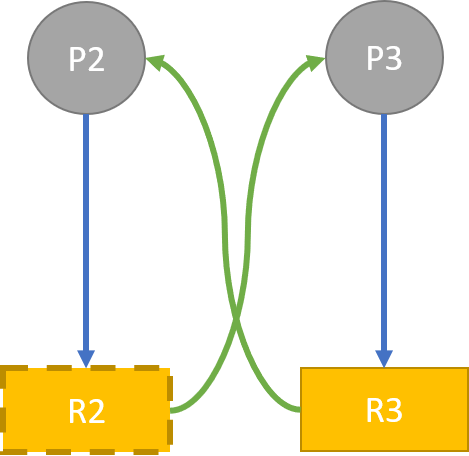
\includegraphics[keepaspectratio, height=0.7\paperheight]{../figs/cap07/exercicio05.png}			
		\end{figure}		
	\end{frame}
				
	\begin{frame}{Questão - Situação 4}
		\begin{itemize}
			\item Recurso R2 é detido pelo processo P3. Processo P2 deseja recurso R2
			\item Recurso R3 é detido pelo processo P2. Processo P3 deseja recurso R3
		\end{itemize}
		\begin{figure}
			\centering
			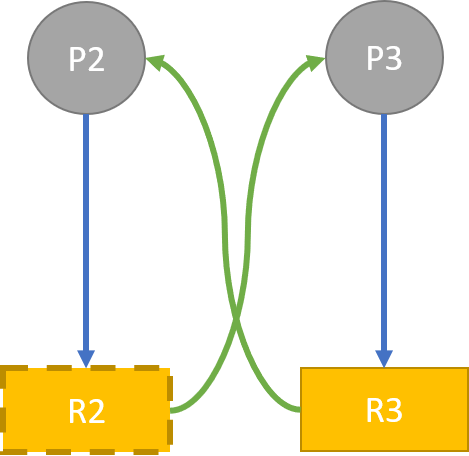
\includegraphics[keepaspectratio, height=0.7\paperheight]{../figs/cap07/exercicio05.png}			
		\end{figure}		
	\end{frame}
	
	\begin{frame}{Recursos com múltiplas instâncias}
		\begin{itemize}
			\item Alguns recursos podem possuir múltiplas instâncias. Neste caso é necessário avaliar se o ciclo causa \textit{deadlock} ou não		
		\end{itemize}
		
		\begin{figure}
			\centering
			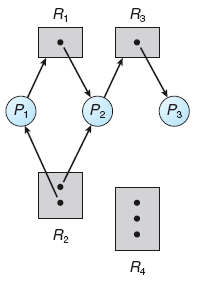
\includegraphics[keepaspectratio, height=0.7\paperheight]{../figs/cap07/recursomulti.png}			
		\end{figure}
	\end{frame}

	\begin{frame}{Múltiplas instâncias - Situação 1}		
		\begin{figure}
			\centering
			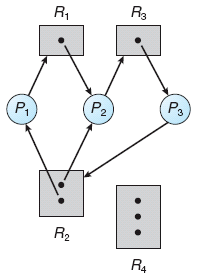
\includegraphics[keepaspectratio, height=0.7\paperheight]{../figs/cap07/recursomulti01.png}			
		\end{figure}
	\end{frame}	
	
	\begin{frame}{Múltiplas instâncias - Situação 2}		
		\begin{figure}
			\centering
			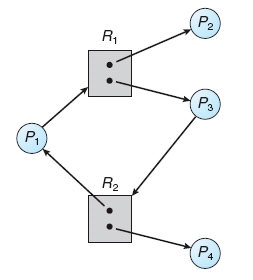
\includegraphics[keepaspectratio, height=0.7\paperheight]{../figs/cap07/recursomulti02.png}			
		\end{figure}
	\end{frame}	
	
	\section{Tratamento de Deadlocks}
	\begin{frame}{Estratégias de tratamento}
		\begin{itemize}
			\item Ignorar completamente o problema
			\item Detecção e recuperação
			\item Evitação dinâmica
			\item Prevenção por negação estrutural
		\end{itemize}
	\end{frame}
	
	\begin{frame}{Algoritmo do Avestruz}
		\begin{itemize}
			\item Estratégia mais econômica.
			\vspace{1em}
			\item Ignorar o problema completamente.
			\vspace{1em}
			\item Decisão baseada em 
			\begin{itemize}
				\item Frequência esperada de impasses
				\item Frequência que o sistema falha por outros motivos
				\item Gravidade do impasse
			\end{itemize}
		\end{itemize}		
	\end{frame}
	
	\begin{frame}{Detecção e recuperação}
		\begin{itemize}
			\item Sistema operacional monitora requisições e liberações de recursos através de um grafo de alocação de recursos
			\vspace{1em}
			\item Em caso de ocorrência de ciclos um processo é finalizado para encerrar o ciclo
			\vspace{1em}
			\item Necessário voltar arquivos para estado original
		\end{itemize}
	\end{frame}
	
	\begin{frame}{Prevenção de deadlock}
		\begin{itemize}
			\item Negação de uma condição de existência do \textit{deadlock}
			\begin{itemize}
				\item Exclusão mútua
				\item Posse e espera
				\item Ausência de preempção
				\item Espera circular
			\end{itemize}
		\end{itemize}
	\end{frame}
	
	\begin{frame}{Exclusão mútua}
		\begin{itemize}
			\item Necessária para o bom funcionamento de recursos compartilhados
			\vspace{1em}
			\item Impossível ser negada para evitar impasses
		\end{itemize}
	\end{frame}
	
	\begin{frame}{Posse e Espera}
		\begin{itemize}
			\item Assegurar que sempre que um processo solicitar um recurso ele não tenha a posse de outro recurso
			\begin{itemize}
				\item Solicitação de todos os recursos necessários de uma só vez
				\item Liberação de recursos retidos antes da solicitação de novos recursos
			\end{itemize}
			\vspace{1em}
			\pause
			\item Problemas
			\begin{itemize}
				\item Má utilização dos recursos
				\item Inanição
			\end{itemize}
		\end{itemize}
	\end{frame}
	
	\begin{frame}{Ausência de preempção}
		\begin{itemize}
			\item Assegurar que um processo não mantenha a posse de um recurso que não está utilizando (preempção forçada)
			\begin{itemize}
				\item Recursos liberados entram na lista de solicitações de recursos do processo			
				\item Facilmente utilizável para recursos como registradores e memória
			\end{itemize}
			\vspace{1em}
			\item Problemas
			\begin{itemize}
				\item Alguns recursos não podem sofrer preempção forçada (impressoras, \textit{locks}, semáforos)
			\end{itemize}			
		\end{itemize}
	\end{frame}
	
	\begin{frame}{Espera circular}
		Estratégias
		\begin{itemize}
			\item Processo pode ter apenas um recurso alocado. Se precisar de um segundo, deve liberar o primeiro
			\item Numeração global de recursos com solicitação em ordem	
		\end{itemize}	
	\end{frame}
	
	\begin{frame}{Resumo das estratégias}
		
		\begin{figure}
			\centering
			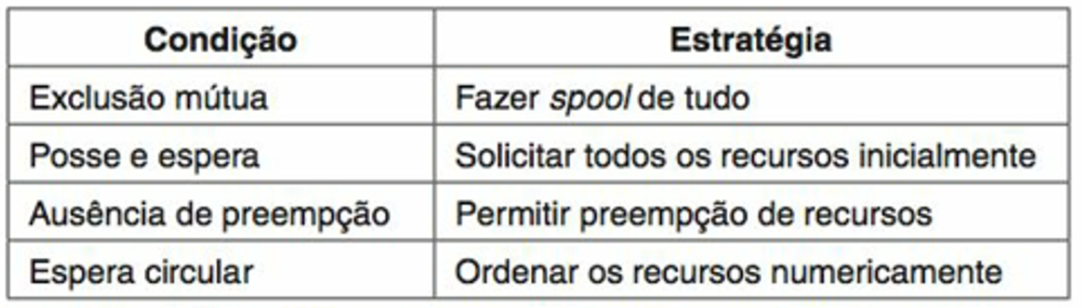
\includegraphics[keepaspectratio, height=0.7\paperheight]{../figs/cap07/estrategias.png}			
		\end{figure}
	\end{frame}
	
	\begin{frame}{Impedimento de deadlock}
		\begin{itemize}
			\item Requer informações adicionais sobre a forma de solicitação dos recursos
			\vspace{1em}
			\item O sistema deve considerar
			\begin{itemize}
				\item Recursos alocados no momento
				\item Recursos disponíveis no momento
				\item Futuras solicitações e liberações de cada processo
			\end{itemize}
			\vspace{1em}
			\begin{itemize}
				\item Algoritmo do banqueiro para um recurso
				\item Algoritmo do banqueiro para múltiplos recursos
			\end{itemize}
		\end{itemize}
	\end{frame}
	
	
	\begin{frame}{Bibliografia}
		\begin{itemize}
			\item SILBERSCHATZ, A.; GALVIN, P. B.; GAGNE, G.. \textbf{Fundamentos de sistemas operacionais: princípios básicos.} Rio de Janeiro: LTC – Livros Técnicos e Científicos, 2013.
			
			\vspace{1em}

			\item TANENBAUM, A.S., WOODHULL, A.S. \textbf{Sistemas Operacionais.} Porto Alegre: Grupo A, 2008.
			
		\end{itemize}
	\end{frame}


	\begin{frame}{}
	\end{frame}	
	
\end{document}
